\begin{appendices}
\chapter{Experiment scenarios}
\label{app:expscenario}

In this appendix, we present the scenario files used for experiment. There are 4 main scenarios in total. \textit{Scenario 1} is used in Section \ref{section:chooseswarmexp}. It has single miner for the experiment. \textit{Scenario 2} is used not only in the Section \ref{section:chooseswarmexp} but also Section \ref{section:swperf}. The number of miner can be changed by adding more node. In this case, we specify it as 25 miners. \textit{Scenario 3} is used in Section \ref{section:chooseswarmexp} to show swarms with multiple level of availability. This can be done by specifying different file size that resides within swarms. The miner is active in node number 101.  Lastly, \textit{Scenario 4} is used in Section \ref{section:expprio}. It specifies the experiment to check user experience in downloading while activating credit mining system. The miner is active in node number 40. 
%\begin{figure}[h!]
%	\begin{adjustwidth}{-2cm}{-2cm}
%		\centering
%		\begin{subfigure}[h]{0.4\textwidth}
%			\centering
%			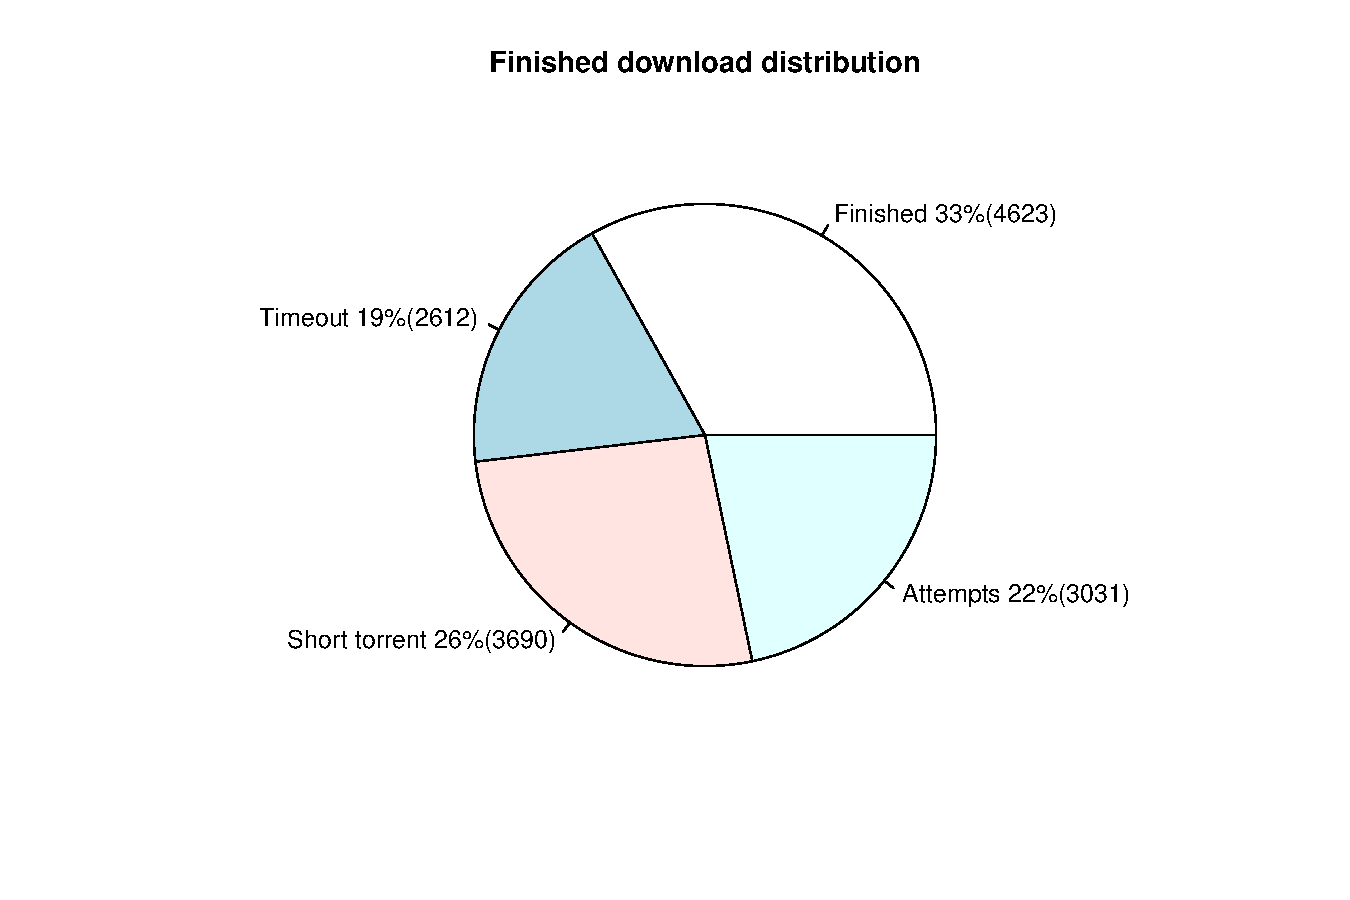
\includegraphics[width=\textwidth]{pics/results/dpredown_t60i30.pdf}
%			\caption{Predownload success percentage}
%			\label{fig:predownprecent}
%		\end{subfigure}
%		\begin{subfigure}[h]{0.4\textwidth}
%			\centering
%			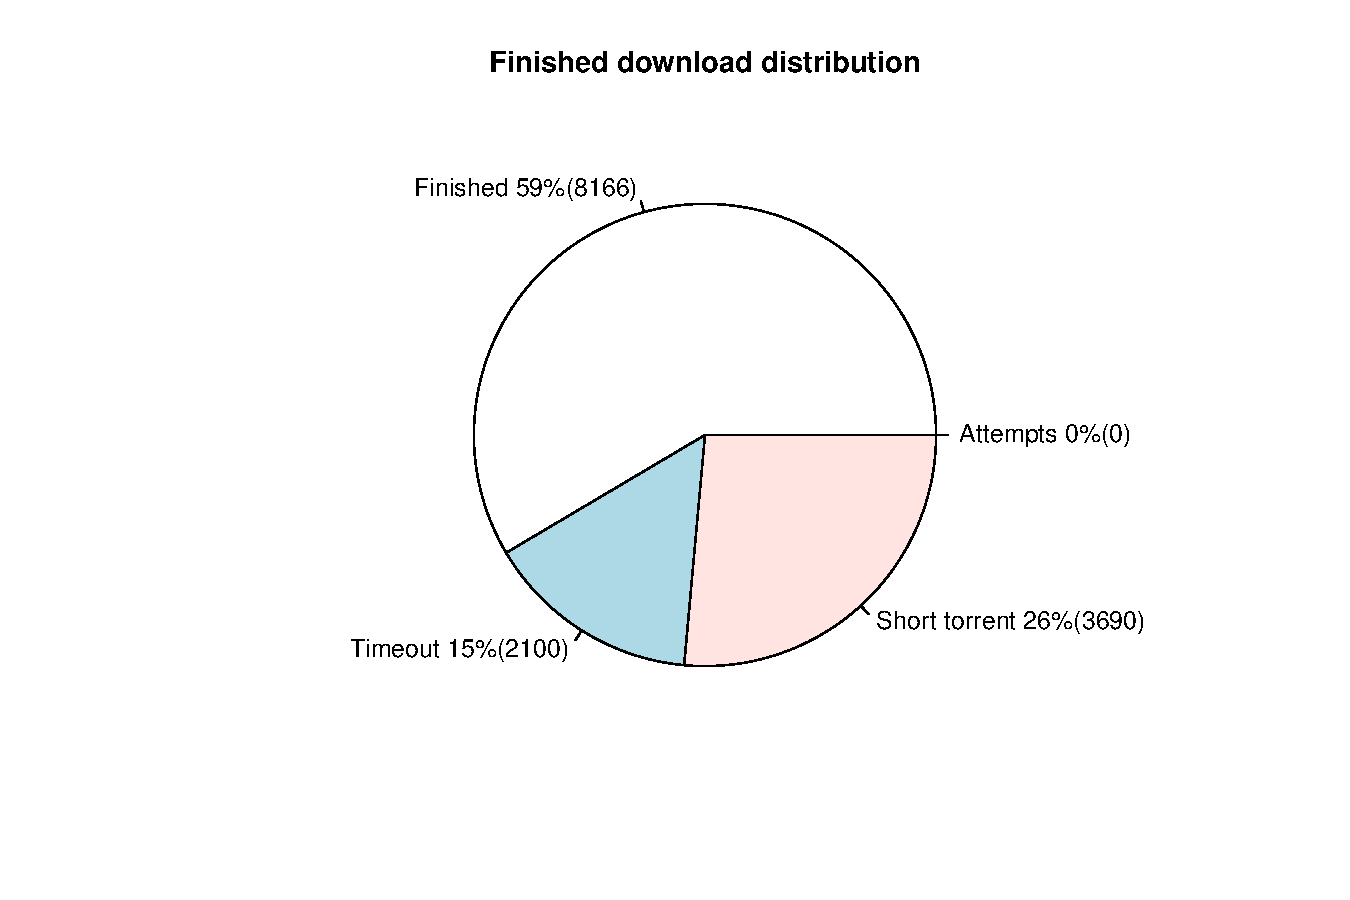
\includegraphics[width=\textwidth]{pics/results/dpredown_sequential.pdf}
%			\caption{Success percentage in sequential piece selection}
%			\label{fig:predownpseq}
%		\end{subfigure}
%		\begin{subfigure}[h]{0.4\textwidth}
%			\centering
%			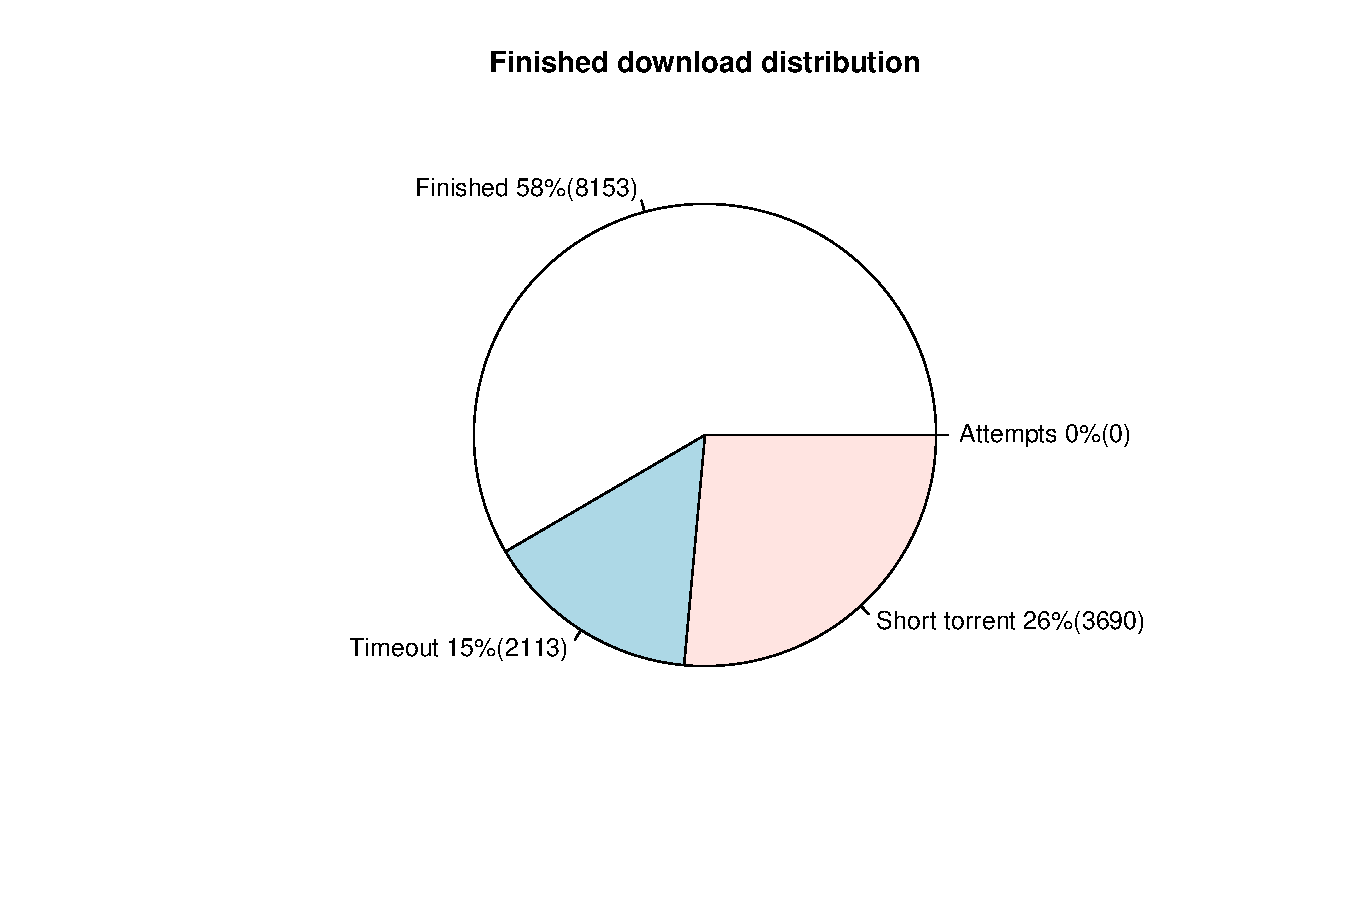
\includegraphics[width=\textwidth]{pics/results/dpredown_random.pdf}
%			\caption{Success percentage in random piece selection}
%			\label{fig:predownprandom}
%		\end{subfigure}
%		\caption{Predownload success percentage for other piece selection approach.}
%	\end{adjustwidth}
%\end{figure}

%\begin{table}[h]
%	\centering
%	\caption{Probability swarm chooser}
%	\begin{adjustwidth}{-2.5cm}{}
%		\begin{tabular}{|c|p{1.5cm}|p{1.5cm}|p{1.5cm}|p{1.5cm}||c|p{1.5cm}|p{1.5cm}|p{1.5cm}|p{1.5cm}|}
%			\hline
%			\rowcolor[HTML]{EFEFEF} 
%			No. & \textit{sc} top 3 (top 6) & \textit{sr} top 3 (top 6) & \textit{sc} on top session & \textit{sr} on top session & No. & \textit{sc} top 3 (top 6) & \textit{sr} top 3 (top 6) & \textit{sc} on top session & \textit{sr} on top session \\ \hline
%			1 & 0  (0) & 0  (0) & 0 & 0 & 19 & 1  (1) & 1  (1) & 1 & 2\\ \hline
%			2 & 0  (0) & 1  (1) & 0 & 1 & 20 & 1  (1) & 1  (1) & 2 & 2\\ \hline
%			3 & 0  (0) & 1  (1) & 0 & 1 & 21 & 1  (2) & 1  (1) & 2 & 2\\ \hline
%			4 & 1  (2) & 1  (1) & 2 & 2 & 22 & 1  (2) & 1  (1) & 2 & 2\\ \hline
%			5 & 1  (2) & 1  (1) & 2 & 1 & 23 & 1  (2) & 1  (1) & 2 & 2\\ \hline
%			6 & 2  (3) & 1  (1) & 3 & 1 & 24 & 1  (1) & 1  (0) & 2 & 2\\ \hline
%			7 & 2  (3) & 1  (1) & 3 & 1 & 25 & 1  (0) & 1  (0) & 2 & 2\\ \hline
%			8 & 1  (2) & 1  (1) & 2 & 2 & 26 & 1  (0) & 1  (0) & 1 & 2\\ \hline
%			9 & 2  (3) & 1  (1) & 3 & 1 & 27 & 1  (0) & 1  (0) & 1 & 1\\ \hline
%			10 & 2  (3) & 1  (1) & 3 & 1 & 28 & 1  (0) & 1  (0) & 1 & 1\\ \hline
%			11 & 2  (3) & 1  (1) & 3 & 1 & 29 & 1  (0) & 1  (0) & 1 & 1\\ \hline
%			12 & 2  (3) & 1  (1) & 3 & 1 & 30 & 1  (0) & 1  (0) & 1 & 1\\ \hline
%			13 & 2  (3) & 1  (1) & 3 & 1 & 31 & 1  (0) & 1  (0) & 1 & 1\\ \hline
%			14 & 1  (2) & 1  (1) & 2 & 1 & 32 & 1  (0) & 1  (0) & 1 & 1\\ \hline
%			15 & 1  (1) & 1  (1) & 2 & 2 & 33 & 0  (0) & 1  (0) & 0 & 1\\ \hline
%			16 & 2  (2) & 1  (1) & 2 & 1 & 34 & 0  (0) & 1  (0) & 0 & 1\\ \hline
%			17 & 1  (2) & 1  (1) & 2 & 1 & 35 & 0  (0) & 1  (0) & 0 & 1\\ \hline
%			18 & 2  (1) & 1  (0) & 2 & 2 & 36 & 0  (0) & 0  (0) & 0 & 0\\ \hline
%		\end{tabular}
%	\end{adjustwidth}
%\end{table}

%Alternative : 

%\begin{table}[h]
%	\centering
%	\caption{Probability swarm chooser (percentage)}
%	\begin{adjustwidth}{-3cm}{}
%		\begin{tabular}{|c|p{1.8cm}|p{1.8cm}|p{1.3cm}|p{1.3cm}||c|p{1.8cm}|p{1.8cm}|p{1.3cm}|p{1.3cm}|}
%			\hline
%			\rowcolor[HTML]{EFEFEF} 
%			Round & \textit{sc} top 3 (top 6) & \textit{sr} top 3 (top 6) & \textit{sc} on top session & \textit{sr} on top session & Round & \textit{sc} top 3 (top 6) & \textit{sr} top 3 (top 6) & \textit{sc} on top session & \textit{sr} on top session \\ \hline
%			1 & 0\%(0\%) & 0\%(0\%) & 0\% & 0\% & 19 & 33\%(33\%) & 33\%(33\%) & 33\% & 67\%\\\hline
%			2 & 0\%(0\%) & 33\%(33\%) & 0\% & 33\% & 20 & 33\%(33\%) & 33\%(33\%) & 67\% & 67\%\\\hline
%			3 & 0\%(0\%) & 33\%(33\%) & 0\% & 33\% & 21 & 33\%(67\%) & 33\%(33\%) & 67\% & 67\%\\\hline
%			4 & 33\%(67\%) & 33\%(33\%) & 67\% & 67\% & 22 & 33\%(67\%) & 33\%(33\%) & 67\% & 67\%\\\hline
%			5 & 33\%(67\%) & 33\%(33\%) & 67\% & 33\% & 23 & 33\%(67\%) & 33\%(33\%) & 67\% & 67\%\\\hline
%			6 & 67\%(100\%) & 33\%(33\%) & 100\% & 33\% & 24 & 33\%(33\%) & 33\%(0\%) & 67\% & 67\%\\\hline
%			7 & 67\%(100\%) & 33\%(33\%) & 100\% & 33\% & 25 & 33\%(0\%) & 33\%(0\%) & 67\% & 67\%\\\hline
%			8 & 33\%(67\%) & 33\%(33\%) & 67\% & 67\% & 26 & 33\%(0\%) & 33\%(0\%) & 33\% & 67\%\\\hline
%			9 & 67\%(100\%) & 33\%(33\%) & 100\% & 33\% & 27 & 33\%(0\%) & 33\%(0\%) & 33\% & 33\%\\\hline
%			10 & 67\%(100\%) & 33\%(33\%) & 100\% & 33\% & 28 & 33\%(0\%) & 33\%(0\%) & 33\% & 33\%\\\hline
%			11 & 67\%(100\%) & 33\%(33\%) & 100\% & 33\% & 29 & 33\%(0\%) & 33\%(0\%) & 33\% & 33\%\\\hline
%			12 & 67\%(100\%) & 33\%(33\%) & 100\% & 33\% & 30 & 33\%(0\%) & 33\%(0\%) & 33\% & 33\%\\\hline
%			13 & 67\%(100\%) & 33\%(33\%) & 100\% & 33\% & 31 & 33\%(0\%) & 33\%(0\%) & 33\% & 33\%\\\hline
%			14 & 33\%(67\%) & 33\%(33\%) & 67\% & 33\% & 32 & 33\%(0\%) & 33\%(0\%) & 33\% & 33\%\\\hline
%			15 & 33\%(33\%) & 33\%(33\%) & 67\% & 67\% & 33 & 0\%(0\%) & 33\%(0\%) & 0\% & 33\%\\\hline
%			16 & 67\%(67\%) & 33\%(33\%) & 67\% & 33\% & 34 & 0\%(0\%) & 33\%(0\%) & 0\% & 33\%\\\hline
%			17 & 33\%(67\%) & 33\%(33\%) & 67\% & 33\% & 35 & 0\%(0\%) & 33\%(0\%) & 0\% & 33\%\\\hline
%			18 & 67\%(33\%) & 33\%(0\%) & 67\% & 67\% & 36 & 0\%(0\%) & 0\%(0\%) & 0\% & 0\%\\\hline
%		\end{tabular}
%	\end{adjustwidth}
%\end{table}

%scoring policy in general similar with sederpolicy. But with considering other factors as well.
%
%in selecting the policy only, the behaviour will similar. Except in edge conditions -> with different availability. Similar seeder ratio.
%=========================================
%choosing best swarm
%case 1
%1. different : seederratio -> expect : similar performance (upload gain) for sr and sc
%scatter, gain graph
%sc gain ~= sr gain
%
%case 2
%2. different : availability -> sc should gather more. seederratio sama, ukuran file beda -> different availability
%scatter, gain graph
%sc gain > sr gain
%
%mention kalau complex experiment ada di akhir (lebih lama)
%DISABLE TRIGGER AND BLACKLIST
%=======================================
%
%increasing Net upload gain
%
%scoring policy
%with trigger < 1.5 times
%blacklist 40mins - 1h recov
%
%
%Statistics (scoring vs seeder ratio): 
%\begin{enumerate}
%	\item Strictly larger Top 3  : 9 (25 \% better)
%	\item Strictly larger Top 6  : 18 (50 \% better)
%	\item Strictly larger top session  : 11
%	\item larger or equal Top 3  : 32 (cover 88 \%)
%	\item larger or equal Top 6  : 35 (cover 97 \%)
%	\item larger or equal top session  : 30
%\end{enumerate}

%\section{Finding best parameters}
%\label{section:cmparamexp}
%The challenge of designing a configurable system is to know what is the effect of the parameters on its performance. Although in the implementation there are many parameters such as the checking period, blacklist threshold and its recovery time, and number of concurrent active swarm in miners, we focused on one that directly related to prospecting method. Therefore, we ended up with two key parameters that need to be evaluated : scoring policy multiplier and the number of downloaded piece in predownload phase.
%
%The experiments in this category will be conducted in both closed environment and the net. In closed environment, we will compare the properties of the swarm observed. The comparison with base performance where credit mining system is not deployed is performed. On the other hand, when launching in the net, custom RSS feed is used. In this case, our focus will be how the credit mining system gain the credit with provided configuration. Both types of experiment run in DAS 4 for 6 hours with 120 nodes. 
%
%\subsection{Multiplier in scoring policy}
%We have mentioned scoring policy in section \ref{section:prospection}. It works by considering swarm properties then gives a score for the properties. There is a weight/multiplier for each properties that stands for its importance. In this experiment we change the multiplier to find out which property and what weight best represent the swarm for prospecting purpose.
%
%We choose the minimum and maximum multiplier by 1 and 5, respectively. In this experiment, a properties is prioritized when the multiplier is 5. On ther other hand, it is not prioritized when the multiplier is 1. Considering there are three properties that need the multiplier, there are six combinations of prioritizing the properties. The algorithm will be executed for every 1 hour. We take note the swarm it choose and compare it to base experiment. The more swarms that selected correctly, the better multiplier combination define the swarm.
%
%\subsection{Number of piece download}
%Another important point of credit mining system is \textit{predownload} phase. By downloading several pieces in start, we put a capital investment hoping that it will act as a mining catalyst. Intuitively, the more capital investment is placed, the higher return will be gained. However, this is not the case in short or medium period. Moreover, another point of \textit{predownload} also to observe peers to get swarm information. Put a large investment on front may become obsolete in next several round.
%
%We start by disabling the predownload, that is, by set zero as number of piece that need to be predownloaded. Next is by set the number as 4, 20, and 50 to represent few, medium, and many piece, respectively. The number of peer and consumed storage are observed. Then, the chosen swarm that relies on the information generated by \textit{predownload} is noted. To have relatively stable number of peer, we will use custom RSS feed to provide us with old but popular content. 
%\subsection{Peer translation accuracy}

%\begin{itemize}
%	\item old one use \textit{net upload gain}. etree.org for two day (48 hour). Test with 1 and half day.
%	\item Best old one is SeederRatio with 5 minute with 1 ratio (gain higher upload gain). Optimal : 3 ratio.
%	\item CM+boost : seederratio, 5 minutes, 3 ratio
%	\item mihai 136 12 hour. runs first. 6dec
%	\item cm 133. 12 hour. runs second. 8dec
%	\item mihai 137, cm 134 : 12 hour. In parallel
%	\item mihai 138 -> cm 136 24h
%	\item mihai 139 & 137 24h par
%\end{itemize}
\begin{lstlisting}[caption={Scenario 1.}]
@0:0 set_master_member 307e....5177
@0:2 start_dispersy {1-106}
@0:20 start_session
@0:60 online
@0:60 reset_dispersy_statistics
@0:60 annotate start-experiment
@0:60 create {1}
@0:61 join {2-20}
@0:62 publish file1gb_1 1524288001 {1}
@0:63 join {21-40}
@0:64 join {41-55}
@0:65 publish file1gb_2 1524288002 {2}
@0:66 publish file1gb_3 1524288003 {3}
@0:67 publish file1gb_4 1524288004 {4}
@0:68 publish file1gb_5 1524288005 {5}
@0:69 publish file1gb_6 1524288006 {6}
@0:70 publish file1gb_7 1524288007 {7}
@0:71 publish file1gb_8 1524288008 {8}
@0:72 publish file1gb_9 1524288009 {9}
@0:73 publish file1gb_10 1524288010 {10}
@5:105 setup_seeder file1gb_2 1524288002 {11}
@5:106 setup_seeder file1gb_3 1524288003 {12-13}
@5:107 setup_seeder file1gb_4 1524288004 {14-16}
@5:108 setup_seeder file1gb_5 1524288005 {17-20}
@5:109 setup_seeder file1gb_6 1524288006 {21-25}
@5:110 setup_seeder file1gb_7 1524288007 {26-31}
@5:111 setup_seeder file1gb_8 1524288008 {32-38}
@5:112 setup_seeder file1gb_9 1524288009 {39-46}
@5:113 setup_seeder file1gb_10 1524288010 {47-55}
@5:114 join {56-105}
@5:115 join {106}
# downloading wave
@10:12 start_download file1gb_1 {56-60}
@10:12 start_download file1gb_2 {61-65}
@10:12 start_download file1gb_3 {66-70}
@10:12 start_download file1gb_4 {71-75}
@10:12 start_download file1gb_5 {76-80}
@10:12 start_download file1gb_6 {81-85}
@10:12 start_download file1gb_7 {86-90}
@10:12 start_download file1gb_8 {91-95}
@10:12 start_download file1gb_9 {96-100}
@10:12 start_download file1gb_10 {101-105}
@20:0 set_boost_settings boosting.ini.1 {106}
@20:2 start_boosting {106}
@20:3 add_source joinedchannel {106}
@2:58:0 reset_dispersy_statistics
@2:59:0 stop
\end{lstlisting}

\begin{lstlisting}[caption={Scenario 2.}]
@0:0 set_master_member 307e....5177
@0:2 start_dispersy {1-130}
@0:20 start_session
@0:60 online
@0:60 reset_dispersy_statistics
@0:60 annotate start-experiment
@0:60 create {1}
@0:61 join {2-20}
@0:62 publish file1gb_1 1524288001 {1}
@0:63 join {21-40}
@0:64 join {41-55}
@0:65 publish file1gb_2 1524288002 {2}
@0:66 publish file1gb_3 1524288003 {3}
@0:67 publish file1gb_4 1524288004 {4}
@0:68 publish file1gb_5 1524288005 {5}
@0:69 publish file1gb_6 1524288006 {6}
@0:70 publish file1gb_7 1524288007 {7}
@0:71 publish file1gb_8 1524288008 {8}
@0:72 publish file1gb_9 1524288009 {9}
@0:73 publish file1gb_10 1524288010 {10}
@5:105 setup_seeder file1gb_2 1524288002 {11}
@5:106 setup_seeder file1gb_3 1524288003 {12-13}
@5:107 setup_seeder file1gb_4 1524288004 {14-16}
@5:108 setup_seeder file1gb_5 1524288005 {17-20}
@5:109 setup_seeder file1gb_6 1524288006 {21-25}
@5:110 setup_seeder file1gb_7 1524288007 {26-31}
@5:111 setup_seeder file1gb_8 1524288008 {32-38}
@5:112 setup_seeder file1gb_9 1524288009 {39-46}
@5:113 setup_seeder file1gb_10 1524288010 {47-55}
@5:114 join {56-105}
@5:115 join {106-130}
# downloading wave
@10:12 start_download file1gb_1 {56-60}
@10:12 start_download file1gb_2 {61-65}
@10:12 start_download file1gb_3 {66-70}
@10:12 start_download file1gb_4 {71-75}
@10:12 start_download file1gb_5 {76-80}
@10:12 start_download file1gb_6 {81-85}
@10:12 start_download file1gb_7 {86-90}
@10:12 start_download file1gb_8 {91-95}
@10:12 start_download file1gb_9 {96-100}
@10:12 start_download file1gb_10 {101-105}
# miners wave
@20:0 set_boost_settings boosting.ini.1 {106-130}
@20:2 start_boosting {106-130}
@20:3 add_source joinedchannel {106-130}
@2:58:0 reset_dispersy_statistics
@2:59:0 stop
\end{lstlisting}
%\begin{figure}[h]
%	\fbox{\theverbbox}
%	\caption{Scenario 1}
%	\label{figapp:scenario}
%\end{figure}

\begin{lstlisting}[caption={Scenario 3.}]
@0:0 set_master_member 307e....5177
@0:2 start_dispersy {1-101}
@0:20 start_session
@0:60 online
@0:60 reset_dispersy_statistics
@0:60 annotate start-experiment
@0:60 create {1}
@0:61 join {2-20}
@0:62 publish file100mb 100428800 {1}
@0:63 join {21-40}
@0:64 join {41-55}
@0:65 publish file300mb 300428800 {2}
@0:66 publish file600mb 600428800 {3}
@0:67 publish file1gb 1000288000 {4}
@0:68 publish file1.3gb 1300288000 {5}
@0:69 publish file1.6gb 1600288000 {6}
@0:70 publish file2gb 2000288000 {7}
@0:71 publish file2.5gb 2500288000 {8}
@0:72 publish file3gb 3000288000 {9}
@0:73 publish file5gb 5000288010 {10}
@5:105 setup_seeder file100mb 100428800 {11-13}
@5:106 setup_seeder file300mb 300428800 {14-16}
@5:107 setup_seeder file600mb 600428800 {17-19}
@5:108 setup_seeder file1gb 1000288000 {20-22}
@5:109 setup_seeder file1.3gb 1300288000 {23-25}
@5:110 setup_seeder file1.6gb 1600288000 {26-28}
@5:111 setup_seeder file2gb 2000288000 {29-31}
@5:112 setup_seeder file2.5gb 2500288000 {32-34}
@5:113 setup_seeder file3gb 3000288000 {35-37}
@5:114 setup_seeder file5gb 5000288010 {38-40}
@5:115 join {56-100}
@5:117 join {101}
# downloading wave
@10:12 start_download file100mb {41-46}
@10:13 start_download file300mb {47-52}
@10:14 start_download file600mb {53-58}
@10:15 start_download file1gb {59-64}
@10:16 start_download file1.3gb {65-70}
@10:17 start_download file1.6gb {71-76}
@10:18 start_download file2gb {77-82}
@10:19 start_download file2.5gb {83-88}
@10:20 start_download file3gb {89-94}
@10:21 start_download file5gb {95-100}
@20:0 set_boost_settings boosting.ini.1 {101}
@20:2 start_boosting {101}
@20:3 add_source joinedchannel {101}
@2:58:0 reset_dispersy_statistics
@2:59:0 stop
\end{lstlisting}

\begin{lstlisting}[caption={Scenario 4.}]
@0:0 set_master_member 307e....5177
@0:2 start_dispersy {1-40}
@0:10 start_session
@0:45 online
@0:46 reset_dispersy_statistics
@0:47 annotate start-experiment
@0:50 create {1}
@0:60 join {2-16}
@0:61 join {17-28}
@0:62 join {29-40}
@1:5 publish the1gb1 1073741821 {1}
@1:6 publish the2gb1 2091474836 {2}
@1:7 publish the2gb2 2104748365 {3}
@1:8 publish the2gb3 2147483691 {4}
@1:13 setup_seeder the1gb1 1073741821 {5-7}
@1:15 setup_seeder the2gb1 2091474836 {9-11}
@1:17 setup_seeder the2gb3 2147483691 {8,12-13}
@1:19 setup_seeder the2gb2 2104748365 {14-16}
@1:30 start_download the1gb1 {17-19}
@1:33 start_download the1gb1 {20}
@4:33 start_download the2gb1 {21-23}
@4:35 start_download the2gb2 {39}
@5:0 set_boost_settings boosting.ini.1 {40}
@5:2 start_boosting {40}
@5:3 add_source joinedchannel {40}
@10:5 start_download the1gb1 {24-27}
@10:6 start_download the2gb1 {24-27}
@10:7 start_download the2gb2 {24-27}
@10:8 start_download the2gb3 {24-27}
@20:30 start_download the1gb1 {28}
@20:32 start_download the2gb1 {29}
@20:33 start_download the2gb1 {30}
@40:31 start_download the2gb3 {40}
@1:20:30 start_download the2gb2 {31-33}
@1:50:30 start_download the2gb1 {34-36}
@2:14:33 start_download the2gb3 {37-38}
@2:58:10 stop
\end{lstlisting}

\end{appendices}